\documentclass[tikz,border=5pt]{standalone}
\usepackage{tikz}
\usetikzlibrary{shapes.geometric,arrows.meta,positioning,calc,backgrounds}

\newcommand{\shapetext}[1]{{\tiny\color{gray!70!black}#1}}

\begin{document}
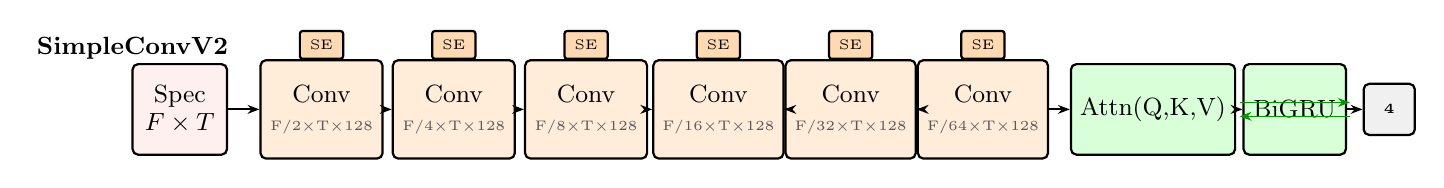
\begin{tikzpicture}[
  x=1.2cm, y=1.2cm,
  font=\small,
  modblock/.style={rectangle, draw, thick, fill=orange!15, rounded corners=2pt, minimum width=1.55cm, minimum height=1.25cm, align=center},
  headblock/.style={rectangle, draw, thick, fill=green!15, rounded corners=2pt, minimum width=1.3cm, minimum height=1.15cm, align=center},
  inputblock/.style={rectangle, draw, thick, fill=red!6, rounded corners=2pt, minimum width=1.2cm, minimum height=1.15cm, align=center},
  outblock/.style={rectangle, draw, thick, fill=gray!12, rounded corners=2pt, minimum width=0.65cm, minimum height=0.65cm, align=center, font=\bfseries\tiny},
  seblock/.style={rectangle, draw, thick, fill=orange!30, rounded corners=1pt, minimum width=0.55cm, minimum height=0.35cm, align=center, font=\tiny},
  arrow/.style={-{Stealth[length=1.5mm]}, thick},
  label/.style={font=\bfseries\small},
]

\node[label] at (-7.3,0.65) {SimpleConvV2};
\node[inputblock] (j-in) at (-6.8,0) {Spec\\[-1pt]$F\times T$};
\node[modblock] (j-b1) at (-5.3,0) {Conv\\[-1pt]\shapetext{F/2$\times$T$\times$128}};
\node[modblock] (j-b2) at (-3.9,0) {Conv\\[-1pt]\shapetext{F/4$\times$T$\times$128}};
\node[modblock] (j-b3) at (-2.5,0) {Conv\\[-1pt]\shapetext{F/8$\times$T$\times$128}};
\node[modblock] (j-b4) at (-1.1,0) {Conv\\[-1pt]\shapetext{F/16$\times$T$\times$128}};
\node[modblock] (j-b5) at (0.3,0) {Conv\\[-1pt]\shapetext{F/32$\times$T$\times$128}};
\node[modblock] (j-b6) at (1.7,0) {Conv\\[-1pt]\shapetext{F/64$\times$T$\times$128}};
\node[seblock] at ([yshift=0.18cm]j-b1.north) {SE};
\node[seblock] at ([yshift=0.18cm]j-b2.north) {SE};
\node[seblock] at ([yshift=0.18cm]j-b3.north) {SE};
\node[seblock] at ([yshift=0.18cm]j-b4.north) {SE};
\node[seblock] at ([yshift=0.18cm]j-b5.north) {SE};
\node[seblock] at ([yshift=0.18cm]j-b6.north) {SE};
\node[headblock] (j-h1) at (3.5,0) {Attn(Q,K,V)};
\node[headblock] (j-h2) at (5.0,0) {BiGRU};
\node[outblock] (j-out) at (6.0,0) {4};
\draw[arrow] (j-in) -- (j-b1);
\draw[arrow] (j-b1) -- (j-b2);
\draw[arrow] (j-b2) -- (j-b3);
\draw[arrow] (j-b3) -- (j-b4);
\draw[arrow] (j-b4) -- (j-b5);
\draw[arrow] (j-b5) -- (j-b6);
\draw[arrow] (j-b6) -- (j-h1);
\draw[arrow] (j-h1) -- (j-h2);
\draw[arrow] (j-h2) -- (j-out);
\draw[arrow, green!60!black, line width=0.5pt] ([yshift=2.5pt,xshift=-1pt]j-h2.west) -- ([yshift=2.5pt,xshift=1pt]j-h2.east);
\draw[arrow, green!60!black, line width=0.5pt] ([yshift=-2.5pt,xshift=1pt]j-h2.east) -- ([yshift=-2.5pt,xshift=-1pt]j-h2.west);

\end{tikzpicture}
\end{document}
